\documentclass[twocolumn,11pt]{article}
\usepackage[margin=1in]{geometry}
\usepackage[T1]{fontenc}
\usepackage[sort]{natbib}
\usepackage{titling}
\usepackage{titlesec}
\usepackage{graphicx}
\usepackage{siunitx}
\usepackage{amsmath,xspace}
\usepackage[backgroundcolor=yellow]{todonotes}
\usepackage[utf8]{inputenc}
\usepackage{bibentry}
\usepackage{float}
\usepackage[ttscale=.875]{libertine}
\usepackage{listings}
\usepackage{libertinust1math}
\usepackage{mdframed} %nice frames
\usepackage[format=plain,
            labelfont={bf,it},
            textfont=it]{caption}
\usepackage{listings}
\usepackage[hyphens]{url}
\usepackage[breaklinks]{hyperref}



\setlength{\columnsep}{5mm}


\author{Daniel Bittman \\ dbittman@ucsc.edu}
\title{NVKV: Building a KV Store for Non-Volatile Memory\\{\Large CMPS278:
Database Design and Implementation: Class Project\\\vspace{-2mm}Instructor: Shel Finkelstein}}

\newcommand{\etal}{\emph{et~al.}\xspace}
\newcommand{\bdb}{Berkeley DB\xspace}
\begin{document}
\biolinum
\maketitle
\libertine 
\renewcommand\ttdefault{lmtt}

\lstset{ 
  backgroundcolor=\color{white},   % choose the background color; you must add \usepackage{color} or \usepackage{xcolor}; should come as last argument
  basicstyle=\ttfamily\footnotesize,        % the size of the fonts that are used for the code
  breakatwhitespace=false,         % sets if automatic breaks should only happen at whitespace
  breaklines=true,                 % sets automatic line breaking
  captionpos=b,                    % sets the caption-position to bottom
  deletekeywords={...},            % if you want to delete keywords from the given language
  escapeinside={\%*}{*)},          % if you want to add LaTeX within your code
  extendedchars=true,              % lets you use non-ASCII characters; for 8-bits encodings only, does not work with UTF-8
  keepspaces=true,                 % keeps spaces in text, useful for keeping indentation of code (possibly needs columns=flexible)
}





\section*{Abstract}


Byte-addressable non-volatile memory (BNVM) will change the memory heirarchy, and
applications must be ready to exploit the advantages afforded by these
technologies while minimizing their weaknesses. Changes in power use
characteristics, consistency requirements, and wear-out means that systems
designed for other memory hierarchies and technologies are not the best fit for
BNVM. We need to think about how to best build systems and applications with the
need for fine-grained consistency, the need to minimize writes to reduce power
and wear-out, and the desire to provide low-latency access to persistent storage
without the operating system getting in the way at every turn.


One example of applications which could be redesigned is key-value stores. We
have built NVKV, a key-value store that attempts to minimize writes while
providing low-latency access, all while remaining consistent regardless of power
cycles and providing backwards compatibility with \bdb. It does this through the
use of transactional memory, or at least what we expect transactional memory to
look like, while minimizing transaction sizes. It provides insert and lookup
functionality with a significant performance improvement over \bdb, while
providing an improvement in consistency safety with respect to power cycles, and
provides better quality of service insert operations. Finally, we demonstrate
that a new Cuckoo hashing variant can reduce data movement and improve the
performance of rehashing significantly.


\section{Introduction}

Byte-addressable non-volatile memory (BNVM) promises to fundamentally change
how applications access persistent
storage~\cite{lee_architecting_2009,fox:2001feram,sttram,wong2010phase,intel3dxpoint},
especially when the memory hierarchy changes to include BNVM along-side DRAM,
and even replacing it entirely.
Changes are expected across the system stack~\cite{condit:sosp09}, with
processors introducing new feature sets, to operating systems providing new I/O
models, to applications redesigned around low-latency persistent memory. Of
particular note is the additional \textit{power} given to middleware
applications---the operating system will provide more direct access to
persistent storage to middleware applications and
libraries~\cite{bittman-ssrctr-17-01}, allowing these applications more control
over their storage techniques and access without operating system interposition.
This has been a long debated topic, and with the advent of BNVM the debate is
coming closer to being settled in favor of applications getting more control and
power.

Of course, with greater power comes greater responsibility, and this is even
more true with BNVM. Data consistency issues threaten most applications, and the
problems of consistency are only magnified with the fine-grained writes of
byte-addressable storage. Whereas writes to DRAM would disappear when power is
cycled, corrupted data structures in BNVM persist across power cycles, meaning
applications must expend additional effort to prevent such corruption that was
not required when the storage hierarchy was separated\footnote{Where we could
rely on block-oriented storage to ease a lot of the difficulty.}. An additional
difficulty is energy use, where prior systems could both buffer writes in DRAM
(which had power usage characteristics that were largely independent of write
bandwidth) and coalesce them to persistent storage. With BNVM, however, the
power scales with write bandwidth at a much higher rate, meaning writes must be
minimized to minimize power. Minimizing writes has the additional benefit of
reducing wear on the memory cells, which is important since many candidate
technologies have significantly lower write endurance than DRAM.

To explore these problems, we have developed NVKV, a non-volatile key-value
store that provides backwards compatibility with the \bdb programming interface.
The prototype implements insert and lookup, although delete would also be trivial
to implement. It organizes and stores data in such a way so that it is easy to
perform all operations using simple and small memory transactions provided by
future software or hardware transactional memory. To support such a design, it
indexes data using a variant of Cuckoo hashing that does not require moving
items when rehashing them. We found that this design allowed the transactions
required to implement insert to be small (fewer than 5 memory access), and that
it was relatively easy to ensure the database could never be corrupted by
unexpected power failures. Furthermore, we found the performance to be
significantly improved over \bdb, likely because our system was designed for
such a memory hierarchy, where \bdb was not. Finally, the Cuckoo hashing variant
we designed resulted in significantly reduced data movement, which is important
for reducing power and wear on BNVM.

The main contributions of this work are:

\begin{enumerate}

\item We motivate the need to reevaluate the design of a key-value store for
BVNM.
\item We build a key-value store, NVKV, which uses transactional
memory to implement updates, and show that is has significantly improved
performance over \bdb.
\item We show that a simple mechanism to minimize writes (simply not reinserting
after expanding the hash table) is viable and does not significantly hurt
overall performance (and in fact, smooths latency spikes caused by expanding the
hash table).
\end{enumerate}



\section{Background}

Non-volatile memory technologies, including phase change memory
(PCM)~\cite{lee_architecting_2009,wong2010phase}, Ferroelectric RAM
(FeRAM)~\cite{fox:2001feram}, and spin-torque transfer RAM (STT-RAM)~\cite{sttram},
among others, promise to fundamentally change the design of our
devices, operating systems, and applications. Although the technologies are
starting to make their way into consumer devices~\cite{intel3dxpoint}, their
full potential will be seen when they replace or exist alongside DRAM on the
memory bus (as byte-addressable non-volatile memory, BNVM).
Such a memory hierarchy will allow the processor, and therefore
applications, to access persistent storage with normal load and store
instructions, bypassing the high-latency I/O operations of the operating system.

The advent of these technologies means that we must build new applications
explicitly designed for them. Whereas existing key-value stores would work when
given access to a file in a file system on BNVM, the result would be sub-optimal
because it would still have the operating system interposing on access to
persistent storage, which is unnecessary for BNVM. Furthermore, the access would
be block oriented, which is irrelevant for these technologies. Finally, the
consistency mechanisms enforced by file systems would be overkill compared to
the more light-weight consistency that could be achieved by a key-value store
designed for BNVM. Together, these all act as additional overhead for key-value
stores that could be avoided by properly redesigning and reevaluating the needs
of such a system. That is a goal of NVKV; understanding the underlying
technology and designing for it.

While this is not new, the particular system model NVKV is built for is. We are
entering an era where we may see a range of persistent memory on the memory bus
from no persistent memory to \textit{only} persistent memory. While some exising
key-value stores are built for persistent memory, they often assume the
existence of DRAM~\cite{echo,Arulraj:2016wbl}. However, IoT devices may soon see
their use of DRAM diminish as more power-friendly technologies come
out~\cite{Jayakumar2014powering}. In fact, from a survey on
papers~\cite{dhiman_pdram:_2009,lee_architecting_2009,xiangyu_dong_nvsim:_2012,qureshi_scalable_2009,Chen_rethinkingdatabase,bedeschi_8mb_2004} discussing
energy consumption of PCM and DRAM, we can see that the energy cost per bit to
write to PCM is 50 times more expensive, but
the idle cost of DRAM is a \textit{billion} times the write cost per bit. This
means that the idle cost of DRAM can only be surpassed by PCM when writing a
billion bits per second. While this is large, it is not unreachable---systems
must be careful to avoid excessive copies and rewrites when using PCM, something 
existing systems do not always optimize for. Finally, since PCM is
extremely energy efficient in read-mostly workloads, it will likely find its
place in IoT devices without DRAM. Thus, key-value stores must be designed for
this all-BNVM model.

\paragraph{Transactional Memory}

Many BNVM systems focus on consistency of data structures due to the
persistent nature of BNVM. When applications store persistent data in
persistent memory, they expect the data to remain consistent with respect to a
set of invariants (e.g. a linked list is valid, etc). However, with the fine
granularity of writes to BNVM and the ability for power failures to strike at
any time, ensuring consistency on BNVM is an important challenge that must be
addressed in new ways.

There are many ways to provide applications with methods for ensuring
consistency, ranging from persisting during shutdown with
battery-backups~\cite{narayanan:asplos12} to write-through caching and careful
ordering with atomics~\cite{bhandari2012implications}, to explicit flushing and
fencing~\cite{condit:sosp09}. While these mechanisms are usable, they range from
being non-portable to being incredibly inefficient. Only explicit flushing is
close to reasonable in terms of both usability and performance, but it has the
same problems as atomic memory accesses without programming language support.
Only with proper language support can persistent memory be both high performance
and easily usable.

The exact form of this language support is still debated, partly because it will
depend on the type of hardware support we see for persistent memory programming.
Hardware support could range from persist barriers to support for transactional
memory. However, existing hardware transactional memory (e.g. in Intel
processors) is deprecated due to bugs. Instead, we are left with enough support
for software transactional memory, which has similar problems as other
approches, namely performance and usability~\cite{stm}. However, hardware
transactional memory \textit{could} be a
reality~\cite{kolli:asplos16,lu:tos16,wang:cal15}---a reality this paper
assumes. Thus, we are focusing on developing a key-value store built for BNVM
with hardware (or software) transactional memory support to ensure consistency.
As an optimization, we additionally make use of weaker consistency mechanisms,
such as fencing and flushing, when transactions would be too heavy-weight for
the updates we are protecting.



\section{Design}


\subsection{Transaction Sizes}

Key points: transactions have limited size, both in space and time. A
transaction cannot take too many instructions, nor have too many memory
accesses. Of course, we're designing under an assumption about how transactions
will work... they may turn out differently. So we're designing pessimistically.

num memory accesses matter more than number of instructions, but the total length
matters too.

We can also optimize certain parts of the code with Os and other parts with
O2/3.


\section{Implementation}

NVKV is shared lib drop-in replacement for BDB.
Describe LoC, cmplexity.
get\_pointer stuff.

what are we ignoring (due to not having bnvm)


\subsection{Consistency Mechanisms}

cuckoo:
order of lookup REALLY matters: reverse order.




cuckoo: each move goes from valid state to valid state with bounded
ops. Worst case the recursive move doesn't complete: still valid.

TXN may be too much overhead. instead, we can use persist-release. We do this
with count, because if the count is off a bit, that's okay. The only time that
happens is power fail, and we can recalculate the count after a fail if we need
it to be perfect.



Calc size of TXNs (num instruction, num of mem access). Also use Os to reduce just
those functions.


TXN, PERSIST\_RELEASE

\subsection{Generated Transaction Code}

As discussed previously, one of the design goals was to reduce the size of
transactions as much as possible. The implementation of \texttt{put} was
designed with this in mind, and is split into two parts: data recording and
indexing. In the data recording phase, the data contained in the key and value
\texttt{DBT}s are saved into NVM. This is currently implemented as an arena-like
allocator that copies each \texttt{DBT} into the database. The data recording
phase does not require transactions since each write maintains correctness; thus
the data recording phase uses only \texttt{persist-release} operations. The
indexing phase, however, uses transactions when updating the hash table.

The design of the cuckoo hash table combined with the choice to not move data
when rehashing means that the hash table uses only two transaction blocks for
\texttt{put}:
\begin{enumerate}
\item \texttt{do\_move}: Copy one bucket to another and zero the source bucket.
\item \texttt{do\_insert}: Write a new key and value pointer into a bucket.
\end{enumerate}
%TODO: make sure we motivate this earlier
Each of these transaction blocks is implemented as a separate function so I
could experiment with the results of using \texttt{-Os} to optimize the blocks
for size rather than speed---an important potential optimization for
transactions that are limited in size or do not scale well with the number of
memory references.

Listings~\ref{lst:moveO3} and~\ref{lst:insertO3} show the generated code for
\texttt{do\_move} and \texttt{do\_insert} respectively when using gcc 7.3.0 on
an Intel x86\_64 processor with native code generation. The result is very
compact, with only the required instructions inside the transaction blocks.
Importantly, for move, the number of memory references is the minimum required to
accomplish the goal of the transaction. However, for insert, the generated code
contains a false dependency: the first line (\texttt{mov -0x68(\%rbp),\%rdi})
does a memory read that does not \textit{need} to be in the transaction block.
Compiler or language support would be required to fully optimize transactions
like this.


\begin{lstlisting}[caption={Transaction code, do\_move, optimized for speed.
Five instructions, five memory accesses (four writes).},label={lst:moveO3}]
     vmovdqu (%rbx), %xmm0
     mov     %r9, 0x10(%r12)
     vmovups %xmm0, (%r12)
     movq    $0x0, 0x10(%rbx)
     movq    $0x0, (%rbx)
\end{lstlisting}

\begin{lstlisting}[caption={Transaction code, do\_insert, optimized for speed.
Four instructions, four memory accesses (three writes).},label=lst:insertO3]
    mov    -0x68(%rbp),%rdi
    mov    %r13,(%rax)
    movq   $0x1,0x10(%rax)
    mov    %rdi,0x8(%rax)
\end{lstlisting}
%$


After applying size optimizations, as shown in Listings~\ref{lst:moveOs}
and~\ref{lst:insertOs}, the insert block is smaller with fewer memory
references. In fact, it no longer contains the false dependency, and contains
the minimum number of memory accesses, but it does have
an extra instruction which again does not \textit{need} to be in the block, thus
further motivating language support. The move operation, however, has
\textit{increased} in size dramatically, containing two instructions which need
not be in the transaction block. However, some of the additional instructions
and memory references come from the fact that gcc chose not to use vector
operations to do the copy in this case, relying instead on simple \texttt{mov}s.
I do not know why this is the case, although I speculate that the reason gcc
chose to do these optimizations was to reduce the number of times these code
blocks appeared in the generated assembly. Whereas the speed-optimized versions
appeared in numerous places throughout the code, the size-optimzed ones were
condensed into one location to reduce size, and therefore gcc was unable to
prove that the \texttt{xmm} registers were available for use. While the result
appears to have more memory references, the two blocks, size and speed optimzed,
touch exactly the same amount of memory (as expected, since they do the same thing).
The important point is that optimizing for size on gcc does not necessarily
optimize for the size of individual blocks of code because the compiler tries to
reduce the size of the program as a whole.




\begin{lstlisting}[caption={Transaction code, do\_move, optimized for size.
Eight instructions, seven memory accesses (five writes).},label=lst:moveOs]
     mov    (%rsi),%rax
     movslq %edx,%rdx
     mov    %rax,(%rdi)
     mov    0x8(%rsi),%rax
     mov    %rdx,0x10(%rdi)
     mov    %rax,0x8(%rdi)
     movq   $0x0,0x10(%rsi)
     movq   $0x0,(%rsi)
\end{lstlisting}

\begin{lstlisting}[caption={Transaction code, do\_insert, optimized for size.
Four instructions, three memory accesses (three writes).},label=lst:insertOs]
     movslq %r8d,%r8
     mov    %rdx,(%rsi)
     mov    %rcx,0x8(%rsi)
     mov    %r8,0x10(%rsi)
\end{lstlisting}





\section{Results and Analysis}

Same test program run linked to each (because portability).

\subsection{Data Movement in the Hash Table}

\begin{figure}
\centering
\hspace*{-0.3in}
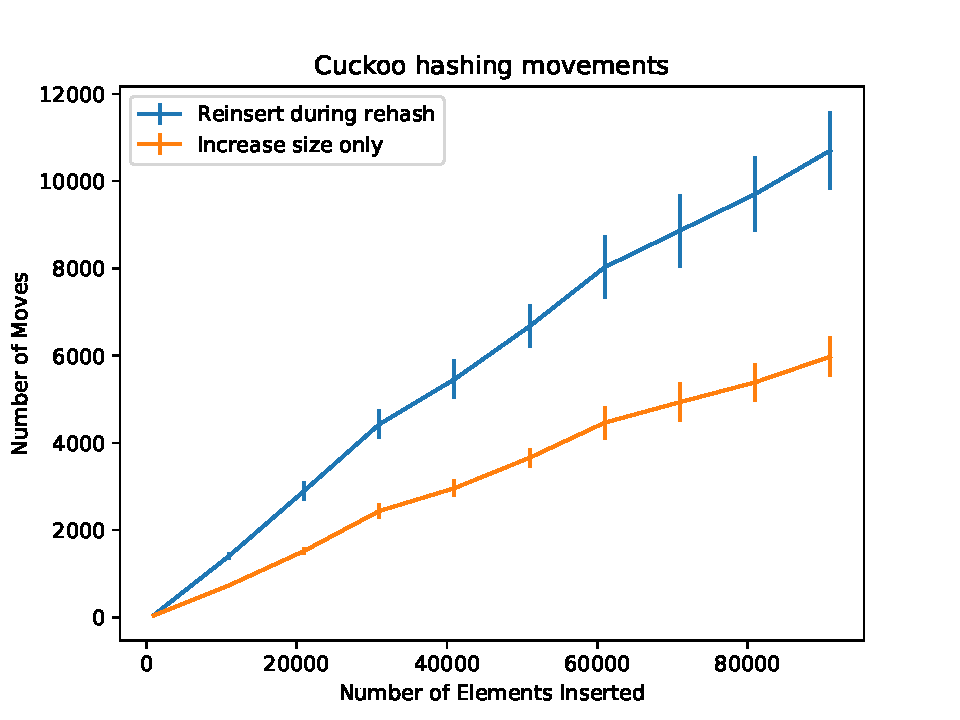
\includegraphics[width=85mm]{fig/moves}
\caption{Movement of buckets during insert for non-reinserting and standard
cuckoo hashing.}
\label{fig:moves}
\end{figure}

The overall number of moves done in the Cuckoo hashing implementation is shown
in Figure~\ref{fig:moves}, and shows that not reinserting elements produces a
significant reduction in the number of moves done during insert operations.
Since Cuckoo hashing is heavily dependent on hash function and workload, these
tests were performed by inserting elements with random keys and counting the
movements done in total, averaged over many runs with different seeds.
The comparison system is a nearly identical
implementation of Cuckoo hashing that reinserts all elements during a rehash.
The error bars show standard deviation, and demonstrate that the non-reinserting
rehashing strategy is less dependent on workload and hash function than standard
cuckoo hashing.

\subsection{Performance}

\begin{figure}
\centering
\hspace*{-0.5in}
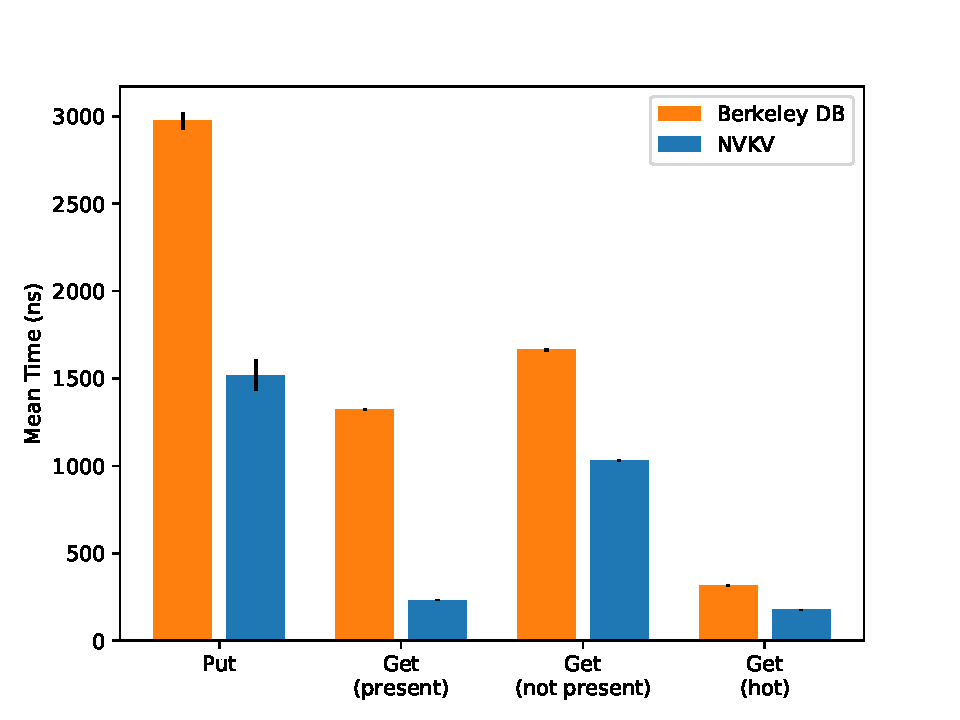
\includegraphics[width=98mm]{fig/perf}
\caption{Latency of various operations for both Berkeley DB and NVKV.}
\label{fig:perf}
\end{figure}

The average latency of insert and lookup operations is shown in
Figure~\ref{fig:perf}. The operations tested are \texttt{put}, which inserts an
element is not present, \texttt{get (present)}, which
looks up an element that is in the database, \texttt{get (not present)}, which
looks up an element that is \textit{not} in the database, and \texttt{get
(hot)}, which looks up the same element repeatedly. The error bars indicate
standard deviation, and are very tight due to the number of tests which were run
on each system. The latency of NVKV operations are significantly lower than the
equivalent Berkeley DB operations due to not needing any system calls in order
to ensure the required consistency and persistence of the insert operations.
Note, however, that the latency of \texttt{put} and \texttt{get (not present)}
is still high for NVKV. In the case of \texttt{put}, this is because of the
overhead of the transactional begin and commit statements along with the
persist-release operations required during the data recording phase of the
insert. In the case of \texttt{get (not present)}, the extra latency comes from
needing to search the hash table at each level that the element \textit{could}
be present.







\begin{figure}
\centering
\hspace*{-0.2in}
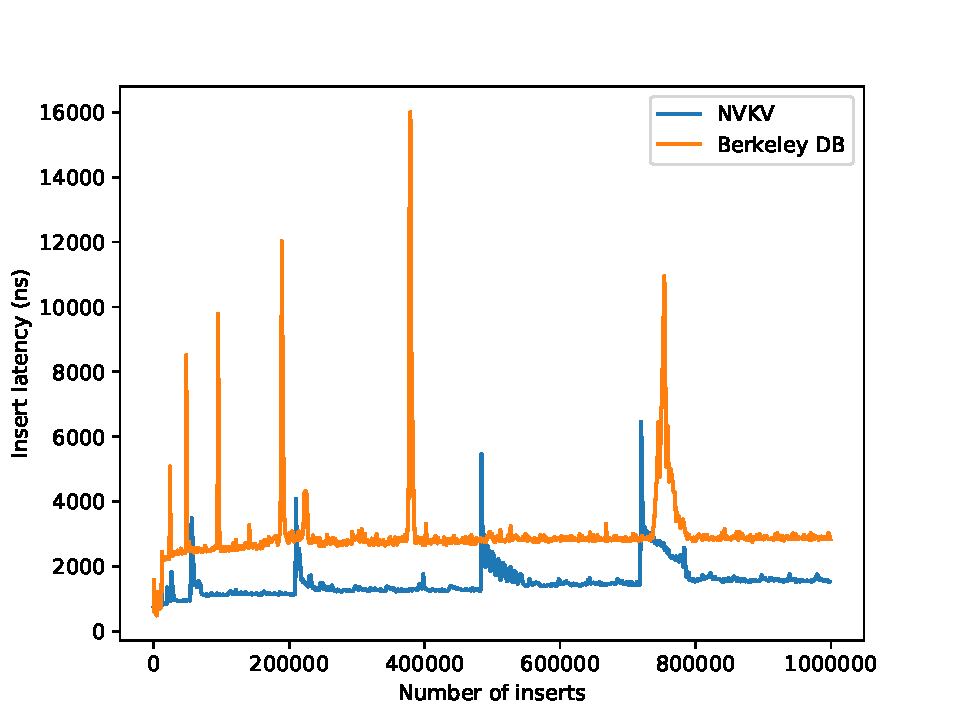
\includegraphics[width=94mm]{fig/line}
\caption{Insert performance as database size grows for both Berkeley DB and
NVKV.}
\label{fig:line}
\end{figure}

Figure~\ref{fig:line} shows the insert performance as a function of the number
of elements in the database for both Berkeley DB and NVKV. As is consistent with
Figure~\ref{fig:perf}, the average insert latency of NVKV is less than Berkeley
DB. Both have significant spikes which are caused by some rearrangement
procedure (in the case of NVKV these correspond to the hash table expansion
procedure).  Note that the NVKV spikes are much smaller, likely due to the
relatively cheap rehashing procedure that does not require reinserting elements.
The NVKV spikes also have a tail to the right of them where the latency remains
significantly above the mean for a time following a hash table expansion. I
expect that this is because the hash table is extremely unbalanced after the
table expansion, resulting in a large number of collisions and movements for
some time after the table is expanded. However, since the elements are always
reinserted at the top level, eventually these collisions will automatically
balance the table as more elements are inserted, amortizing the work of
reinserting during a rehash over future inserts.





\section{Related Work}

\paragraph{BNVM Systems}

There has been a lot of recent work on providing clean and safe abstractions for
non-volatile memory, including data
structures~\cite{coburn:asplos11,hu:atc17,Yang:2015,Venkataraman:2011} and programming
models~\cite{ren:micro15,volos:asplos11,condit:sosp09,guerra:atc12,Narayanan:2012}.
Most of these provide a lower-level interface for applications
to be built atop non-volatile memory and focus on consistency and durability. In contrast, this work does not provide
applications with direct access and control over BNVM data structures; instead,
it provides a key-value interface for applications.

More projects focus on building scalable storage arrays with block-based
non-volatile memory~\cite{Marmol:2014,caulfield:micro10,lim:sosp11,wu:atc15,debnath:vldb10}. We are focusing
on byte-addressable non-volatile memory on the memory bus. Other projects focus
on building full file systems for non-volatile
memory~\cite{wu:asplos94,xu:fast16,xu:sosp17,dulloor:eurosys14}, which is orthogonal to this work because file
systems fullfill different goals than key-value stores.

\paragraph{Hash Tables as BNVM Indexing Structures}

Many have studied the resurgence of hashing as a non-volatile-storage-based
indexing structure due to the random-access,
non-block-oriented nature of the storage technologies. Debnath \etal discuss
improving hash tables for BNVM via several techniques that primarily reduce the
cascading writes effects of cuckoo hashing while maintaining low cache
pressure~\cite{Debnath:2016ht}.
However, they do not focus on making each operation on the table transactionally
consistent nor on reducing the size of the operations which must be protected.
In contrast, while the hash table design in this work could be improved with
some of the same techniques to reduce cascading writes, it focuses on making
each sub-operation serializable and composing them to never leave the table in
an inconsistent state.

\paragraph{Cuckoo Hashing}

There are many improvements to the base cuckoo hashing
algorithm~\cite{Pagh:2004} that can be made, including improving
concurrency~\cite{Li:2014ch}, generalizing cuckoo hashing to d-way
hashing~\cite{Fotakis:hashing}, and cuckoo hashing with CLOCK-style
eviction~\cite{Fan:2013}. These improvements, among the vast numbers of existing
improvements to cuckoo hashing, are not orthogonal to this work, and many could
be used in conjunction with the optimizations and designs presented here.

\paragraph{KV Stores and DBMSs}

There have been numerous projects looking at building key-value stores or
database management systems for non-volatile memories. For example, Arulraj
\etal discuss the implications of BNVM for a DBMS~\cite{Arulraj:2017}. While
many of the lessons there are relevant for key-value stores, many of the design
requirements and implementation details are due to the additional requirements
of a DBMS over a key-value store, and they do not take into account
transactional memory limitations.


Echo is another key-value store designed for non-volatile main
memories~\cite{echo}, however it is also designed with DRAM caching and an
explicit commit operation in mind. In constrast, NVKV persists automatically on
every operation without an interposition of DRAM. A similar problem can be
found in Write-behind logging~\cite{Arulraj:2016wbl}, which uses a novel approach to do logging on
transactions in non-volatile memory. It similarly limits itself to copying
between DRAM and BNVM, as does NVMcached~\cite{Wu:2016}, neither of which
take transactional memory into account.



\section{Future Work}

Future work can be broken down into three broad categories:
\begin{enumerate}
\item \textbf{Expanding}: The functionality of NVKV is extremely limited right
now. There are two major features that are missing that would both be
challenging to implement, but also extremely good candidates for research:
concurrency and larger transactions.

NVKV is currently single-threaded and does not support concurrent operations.
Doing so would be somewhat challenging, since most persistency-safe
transactional memory models do not take concurrent operations into account. The
simple solution is to use locks, resetting them should the power fail. However,
this can limit the multithreaded performance of the application. It would be
interesting to investigate of more fine-grained concurrency would be possible
while remaining consistent across power failures.

Next, NVKV uses transactional memory to ensure its consistency, but it does not
provide support for multi-operation transactions like \bdb does. While support
for such transactions could be implemented in a similar manner, it would be
interesting to determine the most viable way to implement multi-operation
transactions.

\item \textbf{Optimizing}: A significant performance loss for insert is in the
data copy-in phase. Each written word of the data is separately persisted before
the next one is written. If there was language support for a
\textit{persists-with} relationship\footnote{This was my class project in
Programming Languages---defining the math for this to work. It is possible and
can be well defined.} where you could specify that if a particular write $x$
is persisted, then a set of writes $w_0, w_1, ..., w_n$ must also be persisted.
This effectively enforces a visible ordering on persistent writes. It can be
implemented with much higher efficiency than explicit cache-line flushing, and
would significantly improve the data copy-in phase.

Another optimization would be for lookup. If each value were tagged with the
``level'' of the hash table that it was locatable by, and this tag were updated
each time it moved, then the fsck tool could also optimize by calculating the
lowest level required for lookup to check before declaring the item not present.
Alternatively, the fsck tool (which is allowed to optimize the database) could
do the reinsert of each item in the table, as long as it first made a backup.

\item \textbf{Exploring}: Finally, the Cuckoo hashing variant presented here has
merit for further exploration and research. An obvious path would be to explore
how other variants of Cuckoo hashing (which, for example, increase the load factor that
the table can tolerate) can interoperate with the no-reinsertion while rehashing
scheme. Finally, a more detailed analysis of this scheme should be done.

\end{enumerate}

\section{Conclusion}



\section*{Availability}
The code and data for this project can be found
at \url{https://github.com/dbittman/cmps278}.

\section*{Acknowledgements}

Thanks to Matt Bryson for helping collect some of the papers for energy use
in PCM and DRAM (these results were used for another project in the SSRC in a
more detailed manner, but are mentioned here because they are relevant to
the motivation).

\bibliographystyle{plain}
\bibliography{bib/csrg,main,pcm_hardware}

\end{document}

